% chinthakawk@gmail.com

\documentclass[compress]{beamer} %this is to use copressed header from the
\usepackage{etex}
\usepackage{beamerthemeshadow} %our theme, later you can change it
\usepackage[frenchb]{babel}
\usepackage{fancyhdr} % Required for custom headers
\usepackage[utf8]{inputenc}
\usepackage[lined,boxed]{algorithm2e}
\usepackage[all]{xy}
\usepackage{animate} %need the animate.sty file
\graphicspath{{./Figure/}} 
% editing header
\setbeamertemplate{headline}
{
  \leavevmode%
  \hbox{%
  \begin{beamercolorbox}[wd=.5\paperwidth,ht=2.25ex,dp=1.8ex,leftskip=1em,left]{section in head/foot}%
    \usebeamerfont{subsection in head/foot}\hspace*{5ex}\insertsectionhead
  \end{beamercolorbox}%
  \begin{beamercolorbox}[wd=.5\paperwidth,ht=2.25ex,dp=1.8ex,left,leftskip=1em]{subsection in head/foot}%
    \usebeamerfont{section in head/foot}\insertshorttitle\hspace*{2ex}
  \end{beamercolorbox}}%
  \vskip0pt%
}

% editing footer
\setbeamertemplate{footline}
{
  \leavevmode%
  \hbox{%
  \begin{beamercolorbox}[wd=.5\paperwidth,ht=2.25ex,dp=1ex,right]{author in head/foot}%
    \usebeamerfont{author in head/foot}\insertshortauthor\hspace*{2ex}
  \end{beamercolorbox}%
  \begin{beamercolorbox}[wd=.5\paperwidth,ht=2.25ex,dp=1ex,right]{date in head/foot}%
    \usebeamerfont{date in head/foot}\insertshortdate{}\hspace*{2em}
    \insertframenumber{} / \inserttotalframenumber\hspace*{2ex} 
  \end{beamercolorbox}}%
  \vskip0pt%
}
\definecolor{orange}{rgb}{1,0.5,0}
\definecolor{darkgreen}{rgb}{0,0.5,0}
\definecolor{darkblue}{rgb}{0,0,0.5}

\def\etal{et al.\ }
\def\ie{i.e.\ }
\def\eg{e.g.\ }

%insert 2 figures on a row
\newcommand{\insertTwoF}[4]{
  \begin{figure}[h!]
    \centering
    \begin{minipage}{#4\linewidth}
    \includegraphics[width=\linewidth]{#1}
    \end{minipage}
    \begin{minipage}{#4\linewidth}
    \includegraphics[width=\linewidth]{#2}
    \end{minipage}
      \caption{#3}
  \end{figure}  
}

\newcommand{\insertF}[3]{
  \begin{figure}[h!]
    \centering
    \begin{minipage}{#3\linewidth}
    \includegraphics[width=\linewidth]{#1}
    \end{minipage}  
      \caption{#2}
  \end{figure}  
}

%enable numbering captions for the images
\setbeamertemplate{caption}[numbered]


\begin{document}

 \title{Décors3D} 
 \section{title}
 %title page
 \begin{frame}
\titlepage
    \centering
    \begin{minipage}{0.4\textwidth}
    \begin{flushleft} \large
    \emph{Auteurs:}\\
    T. Dalens, A. Dhobb,\\
    B. Giroud, M. Keribin,\\
    T. Rebele, M. Xu\\
    \end{flushleft}
    \end{minipage}
    \begin{minipage}{0.4\textwidth}
    \begin{flushright} \large
    \emph{Cours :}\\
    SI 381\\
    \emph{Encadrants :}\\
    M. Roux
    S. Ladjal
    \end{flushright}
    \end{minipage}\\[3cm]
 \end{frame}
\section{Segmentation en plans}

 
 \begin{frame}
 \frametitle{Architecture}
 \textbf{Entr�e :}  Une vid�o \\ 
 
 \textbf{Sortie :}  Une s�rie de frames clés pour chaque plan de la vid�o \\
 
 \end{frame}

 \begin{frame}
 \frametitle{Histogramme HSV}
 \insertTwoF{Fig/hsv1.jpg}{Fig/hsv2.jpg}{d�composition selon H,S et V}{0.3}
 \end{frame}
 
 \begin{frame}
 \frametitle{Histogramme HSV}
 On calcule un histogramme HSV normalisé sur 16 bins pour chaque frame : 8 bins pour H, 4 pour S et 4 pour V.\\
 \vspace{1cm}
 \verb![Rasheed, Shah, CVPR 2003]!\\
 \end{frame}
 
 \begin{frame}
 \frametitle{D�tection des changements plans}
 
 \textbf{Principe :} On compare les histogrammes entre 2 frames consécutives. Si l'intersection entre ces 2 histogrammes est inf�rieure � un certain seuil, cela indique qu'il y a un changement de plan. \\
 \[d_{intersection}(H_{1},H_{2}) = \sum_{i} min(H_{1}(i),H_{2}(i))\]
 
 \end{frame}
 
 
 \begin{frame}
 \frametitle{Extraction de frames cl�s d'une m�me sc�ne}
 \textbf{Principe :}
\begin{itemize} 
\item{On fixe un deuxi�me seuil}
\item{On extrait la premi�re frame du plan qui est la frame de r�f�rence}
\item{Pour chaque frame de ce plan, on calcule l'intersection de son histogramme avec l'histogramme de la frame de r�f�rence}
\item{Si l'intersection est inf�rieure � notre seuil, on extrait cette frame qui devient la nouvelle frame de r�f�rence}
\end{itemize}
\end{frame}

\begin{frame}
 \frametitle{Extraction de frames cl�s d'une m�me sc�ne}
\end{frame}

 

 
 
 
 \section{Inpainting}
 %MODIFIER ICI
 \section{Modélisation 3D}
 %MODIFIER ICI
 \section{Examples}
 
 \begin{frame}
  \frametitle{Exemples d'images}
  \insertF{Fig/chat1.jpg}{petit chaton 1}{0.3}
  \insertF{Fig/chat2.jpg}{petit chaton 2}{0.3}
 \end{frame}
 
 \begin{frame}
  \frametitle{Exemples d'images}
  \insertTwoF{Fig/chat1.jpg}{Fig/chat2.jpg}{petits chatons}{0.4}
 \end{frame}
 \begin{frame}
   Exemples de table des matières

 \begin{enumerate}


   \item partie 1
   \item partie 2
   \item partie 3
   
 \end{enumerate}

 
 \end{frame} 
 
 \begin{frame}
 exemples de texte avec \emph{emphase}, \textbf{gras}, maths $x_{n+1}^2=0$ et encore maths
 \[
 \frac{\sin(x)}{x} = 6
 \]
 \end{frame}
 
\end{document}

 
 % please change content in the following files (with ending .tex)
 \section{Introduction}
%%%%%%%%%%%%%%%%%%%
 % Frame plan
\begin{frame}
  \frametitle{Plan de la présentation}
  \begin{itemize}
  \item Introduction
  \end{itemize}
  \begin{enumerate}
  \item Segmentation
  \item Inpainting 2D+t
  \item Reconstruction 3D
  \end{enumerate}
  \begin{itemize}
  \item Conclusion
  \item Démonstration
  \end{itemize}
  

\end{frame}



 %%%%%%%%%%%%%%%%%%%
 % Frame presentation of the programm : idee, what he does
 \begin{frame}
   \frametitle{Contexte}
   
   \begin{itemize}
   
   \item Industrie du film est très importante et donne de nombreux produits dérivés
   	\begin{itemize}
   	\item Parodies
   	\item Industrie des jeux vidéos
   	\item Reconstruction décor réel en virtuel
   	\end{itemize}
   
   \item État de l'art
   	\begin{itemize}
   	\item Indexation
   	\item Détection de personnages
   	\item Inpainting 2D+t
   	\item Reconstruction 3D d'objets

   	\end{itemize}
   	
   \item Notre idée
   	\begin{itemize}
   	\item Supprimer les personnages pour obtenir les décors des films
   	\end{itemize}
   
   \end{itemize}
 
 \end{frame}


  %%%%%%%%%%%%%%%
  % Frame purposes, how to use it
 \begin{frame}
   \frametitle{Objectif}
   
   \begin{itemize}
   \item Obtenir le décor des films
   	\begin{itemize}
   	\item Sous format 3D si possible
   	\item En 2D sinon
   	\end{itemize}
   	
   \item Fonctionnement idéal
   	\begin{itemize}
   	\item Donner un film en entrée
   	\item Détecter les différents points de vue
   	\item Grouper les scènes d'un même décor
   	\item Supprimer les personnages
   	\item Obtenir un maillage 3D du décor
   	\end{itemize}
   
   \item Problèmes à résoudre
  	\begin{itemize}
	\item Présence de personnages devant le décor
	\item Définition du décor
	\item Scène fixes
  	\end{itemize}

   \end{itemize}
	
 \end{frame}
 
 %%%%%%%%%%%%%%%%%%%
 % Frame architecture
\begin{frame}
  \frametitle{Architecture}
  \insertF{Fig/architectureGlobale.png}{Architecture de notre programme}{1}

\end{frame}


 %%%%%%%%%%%%%%%
  % Frame demonstration
 \begin{frame}
   \frametitle{Démonstration}
   \begin{figure}
   
\includegraphics[width=0.5\textwidth]{Fig/workInProgress.png}
   \end{figure}

 \end{frame}
  \section{Segmentation}
 %MODIFIER ICI
 %%%%%%%%%%%%%%%
 % Frame Section title
 \begin{frame}
 \title{Segmentation}
 \titlepage

    \begin{minipage}{0.3\textwidth}
    \begin{flushleft} \large
    \emph{Binôme :}\\
    T. Dalens\\
    A. Dhobb
    \end{flushleft}
    \end{minipage}
    \begin{minipage}{0.5\textwidth}
    \begin{flushright} \large
    \begin{figure}
    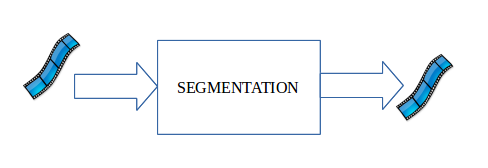
\includegraphics[width=1.4\textwidth]{Fig/architectureSectionSegmentation.png}
    \end{figure}
    \end{flushright}
    \end{minipage}\\[3cm]
    
 \end{frame}
 
 
%%%%%%%%%%%%%%%
 % Frame Architecture inpainting
\begin{frame}
  \frametitle{Architecture du programme}
  \insertF{Fig/architectureSegmentationFinale.png}{Architecture de la partie Segmentation}{0.9}
  
\end{frame} 
 
 


 %%%%%%%%%%%%%%%
 \begin{frame}
 \frametitle{Histogramme HSV}
 \insertTwoF{Fig/hsv1.jpg}{Fig/hsv2.jpg}{décomposition selon H,S et V}{0.3}
 \end{frame}
 
 \begin{frame}
 \frametitle{Histogramme HSV}
 On calcule un histogramme HSV normalisé sur 16 bins pour chaque frame : 8 bins pour H, 4 pour S et 4 pour V.\\
 \vspace{1cm}
 \verb![Rasheed, Shah, CVPR 2003]!\\
 \end{frame}
 
 \begin{frame}
 \frametitle{Détection des changements plans}
 
 \textbf{Principe :} On compare les histogrammes entre 2 frames consécutives. Si l'intersection entre ces 2 histogrammes est inférieure à un certain seuil, cela indique qu'il y a un changement de plan. \\
 \[d_{intersection}(H_{1},H_{2}) = \sum_{i} \min(H_{1}(i),H_{2}(i))\]
 
 \end{frame}
 
 
 \begin{frame}
 \frametitle{Extraction de frames clés d'un même plan}
 \textbf{Principe :}
\begin{itemize} 
\item{On fixe un deuxième seuil}
\item{On extrait la première frame du plan qui est la frame de référence}
\item{Pour chaque frame de ce plan, on calcule l'intersection de son histogramme avec l'histogramme de la frame de référence}
\item{Si l'intersection est inférieure à notre seuil, on extrait cette frame qui devient la nouvelle frame de référence}
\end{itemize}
\end{frame}

\begin{frame}
 \frametitle{Extraction de frames clés d'un même plan}
 \insertF{Fig/Spiderman.jpg}{Frames clés d'un plan de \emph{Spiderman 2}}{1}
\end{frame}



 %%%%%%%%%%%%%%%
  % Frame demonstration
 \begin{frame}
   \frametitle{Démonstration}
   \begin{figure}
   
\includegraphics[width=0.5\textwidth]{Fig/demoInProgress.png}
   \end{figure}

 \end{frame}
  \section{Inpainting}
 %MODIFIER ICI
 %%%%%%%%%%%%%%%
 % Frame Section title
 \begin{frame}
 \title{Inpainting}
 \titlepage

    \begin{minipage}{0.3\textwidth}
    \begin{flushleft} \large
    \emph{Binôme :}\\
    M. Keribin\\
    T. Rebele
    \end{flushleft}
    \end{minipage}
    \begin{minipage}{0.5\textwidth}
    \begin{flushright} \large
    \begin{figure}
    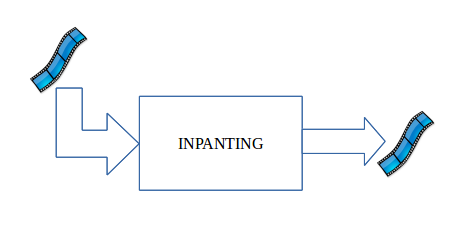
\includegraphics[width=1.4\textwidth]{Fig/architectureSectionInpainting.png}
    \end{figure}
    \end{flushright}
    \end{minipage}\\[3cm]
    
 \end{frame}



 %%%%%%%%%%%%%%%
 % Frame Architecture inpainting
\begin{frame}
  \frametitle{Architecture du programme}
  \insertF{Fig/architectureInpainting.png}{Architecture de la partie Inpainting}{1}

\end{frame}



 %%%%%%%%%%%%%%%
 % Frame KeyPoints
\begin{frame}
  \frametitle{Keypoints}
  
  \begin{itemize}
  \item SURF
  	\begin{itemize}
  	\item Inspiré des SIFTs
  	\item Utilise ondelettes de Haar
  	\end{itemize}
  	
  \item GFTT (Harris)
	\begin{itemize}
  	\item Détection des coins
  	\end{itemize}
  	
  \item Canny
    \begin{itemize}
  	\item Détection des contours
  	\end{itemize}
  	
  \end{itemize}
    \insertF{Fig/cannyPoints.png}{Points de Canny}{0.4}


\end{frame}



 %%%%%%%%%%%%%%%
 % Frame create trace
\begin{frame}
  \frametitle{Trace}
  \begin{itemize}
  \item Recherche de correspondances entre points
  	\begin{itemize}
  	\item Sélection des keypoints
  	\item Recherche dans le voisinage frame suivante
  	\end{itemize}
  \item Estimer l'homographie
  \item Trace
  	\begin{itemize}
  	\item Créer et continuer la trace
  	\item Classifier la trace
  	\begin{itemize}
  		\item fixe
  		\item mobile
  		\item indéterminé
  	\end{itemize}
  	\end{itemize}
  \end{itemize}
  
    \insertF{Fig/cannyKeypoints.png}{Mise en évidence des keypoints et de la trace}{0.4}


\end{frame}


 %%%%%%%%%%%%%%%
 % Frame inpainting principe
\begin{frame}
  \frametitle{Remplissage}
  
  \begin{itemize}
  \item Classifier les zones
  	\begin{itemize}
  	\item fixe $\leftrightarrow$ noir
  	\item mobile $\leftrightarrow$ couleur du fond
  	\end{itemize}
  \item Remplir quand le point devient fixe  
  \end{itemize}

  \begin{figure}
  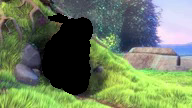
\includegraphics[width=0.45\textwidth]{Fig/bunny2-masked.png}
  
\includegraphics[width=0.45\textwidth]{Fig/bunny1-original.png}
  \caption{Principe de l'inpainting 2D + t}
  \end{figure}
   
\end{frame}


 %%%%%%%%%%%%%%%
  % Frame demonstration
 \begin{frame}
   \frametitle{Démonstration}
   \begin{figure}
   
\includegraphics[width=0.5\textwidth]{Fig/workInProgress.png}
   \end{figure}

 \end{frame}
 
 \section{Modélisation 3D}
 %MODIFIER ICI

 \section{Conclusion}
%%%%%%%%%%%%%%%
 % Frame Section title
 \begin{frame}
 \title{Conclusion}
 \titlepage

 \end{frame}
 
 
 
%%%%%%%%%%%%%%%%%%%
 % Frame conclusion
\begin{frame}
\frametitle{Conclusion}

\end{frame}


%%%%%%%%%%%%%%%%%%%
 % Frame show the result of demo in live
 \begin{frame}
 \frametitle{Résultat de la démonstration}
 \begin{figure}
   
\includegraphics[width=0.5\textwidth]{Fig/workInProgress.png}
   \end{figure}

\end{frame}

%%%%%%%%%%%%%%%%%%%
 % Frame question
 \begin{frame}
 \frametitle{Questions}
 \begin{figure}
 
\includegraphics[width=0.5\textwidth]{Fig/question.jpg}
 \end{figure}

\end{frame}


 \section{Examples}
 
 \begin{frame}
  \frametitle{Exemples d'images}
  \insertF{Fig/chat1.jpg}{petit chaton 1}{0.3}
  \insertF{Fig/chat2.jpg}{petit chaton 2}{0.3}
 \end{frame}
 
 \begin{frame}
  \frametitle{Exemples d'images}
  \insertTwoF{Fig/chat1.jpg}{Fig/chat2.jpg}{petits chatons}{0.4}
 \end{frame}
 \begin{frame}
   Exemples de table des matières

 \begin{enumerate}


   \item partie 1
   \item partie 2
   \item partie 3
   
 \end{enumerate}

 
 \end{frame} 
 
 \begin{frame}
 exemples de texte avec \emph{emphase}, \textbf{gras}, maths $x_{n+1}^2=0$ et encore maths
 \[
 \frac{\sin(x)}{x} = 6
 \]
 \end{frame}

 
\end{document}
